\label{3_algoritmo_genetico}

O pseudocódigo tradicional de um algoritmo evolutivo pode ser dado por \cite{algoritmopseudo}:

\begin{algorithm}[H]
$\textbf{AG(} fitness \textbf{)}$
\Begin{
	$P \gets InicializarPopulacao(fitness)$\;
	$P.fitness()$\;
	$t = 0$\;
	\While{t < número de gerações} {
		$Pais \gets Selecao(P)$\;
		$Filhos \gets Crossover(Pais)$\;
		$P \gets P \cup Filhos$\;
		$Mutacao(P)$\;
		$P.fitness()$\;
		$P \gets Sobrevivem(P)$\;
	}
}
\caption{Pseudocódigo de um Algoritmo Evolutivo.}
\label{alg:ae}
\end{algorithm}

Cada uma destas funções principais pode ser feita de diferentes maneiras. No entanto, tais implementações independem do problema a ser resolvido, o que torna sua confecção e manutenção bem mais simples.

Para que este trabalho não fugisse muito de seu escopo, que é o de resolver problemas, as decisões feitas para o AG tentaram ser as mais simples possíveis frente à literatura existente.

\section{Parâmetros de entrada}

O AG possui uma série de algoritmos de entrada. No entanto, excetuando-se os parâmetros específicos de cada problema (como os associados à função de fitness ou ao tipo de indivíduo que comporá a população), restam um total de 4 parâmetros:

\begin{itemize}
	\item O número de indivíduos na população ($\mu$);
	\item O número de gerações ($NGEN$);
	\item A probabilidade de crossover ($p_c$);
	\item A probabilidade de mutação ($p_m$).
\end{itemize}

As variáveis $p_c$ e $p_m$ serão discutidas a seguir. O valor de $NGEN$ variou de acordo com o problema e com sua complexidade, mas foi padronizado um valor empírico de 120 gerações para cada execução do AG. O valor de $\mu$ ficou padronizado como 100.

\section{Seleção dos pais}

A escolha dos pais foi feita ordenando a geração em função de seu valor de fitness, com os pais sendo pareados sequencialmente, dois a dois.

\section{Recombinação / Crossover}

Escolhidos os pais, avalia-se, com probabilidade $p_c$, se eles serão cruzados. Se sim, seus materiais genéticos serão misturados por uma ação chamada \emph{crossover}.

O crossover envolve a quebra da sequência de genes de dois indivíduos em uma mesma secção, com a subsequente troca de material na região delimitada por esta secção. Este trabalho se utilizou do crossover em dois pontos, o qual divide as sequências em duas partes distintas, ocorrendo troca do material genético entre estas partes. Tal ação é mostrada na figura \ref{fig:evolution-framework}.

\begin{figure}[ht!]
    \centering 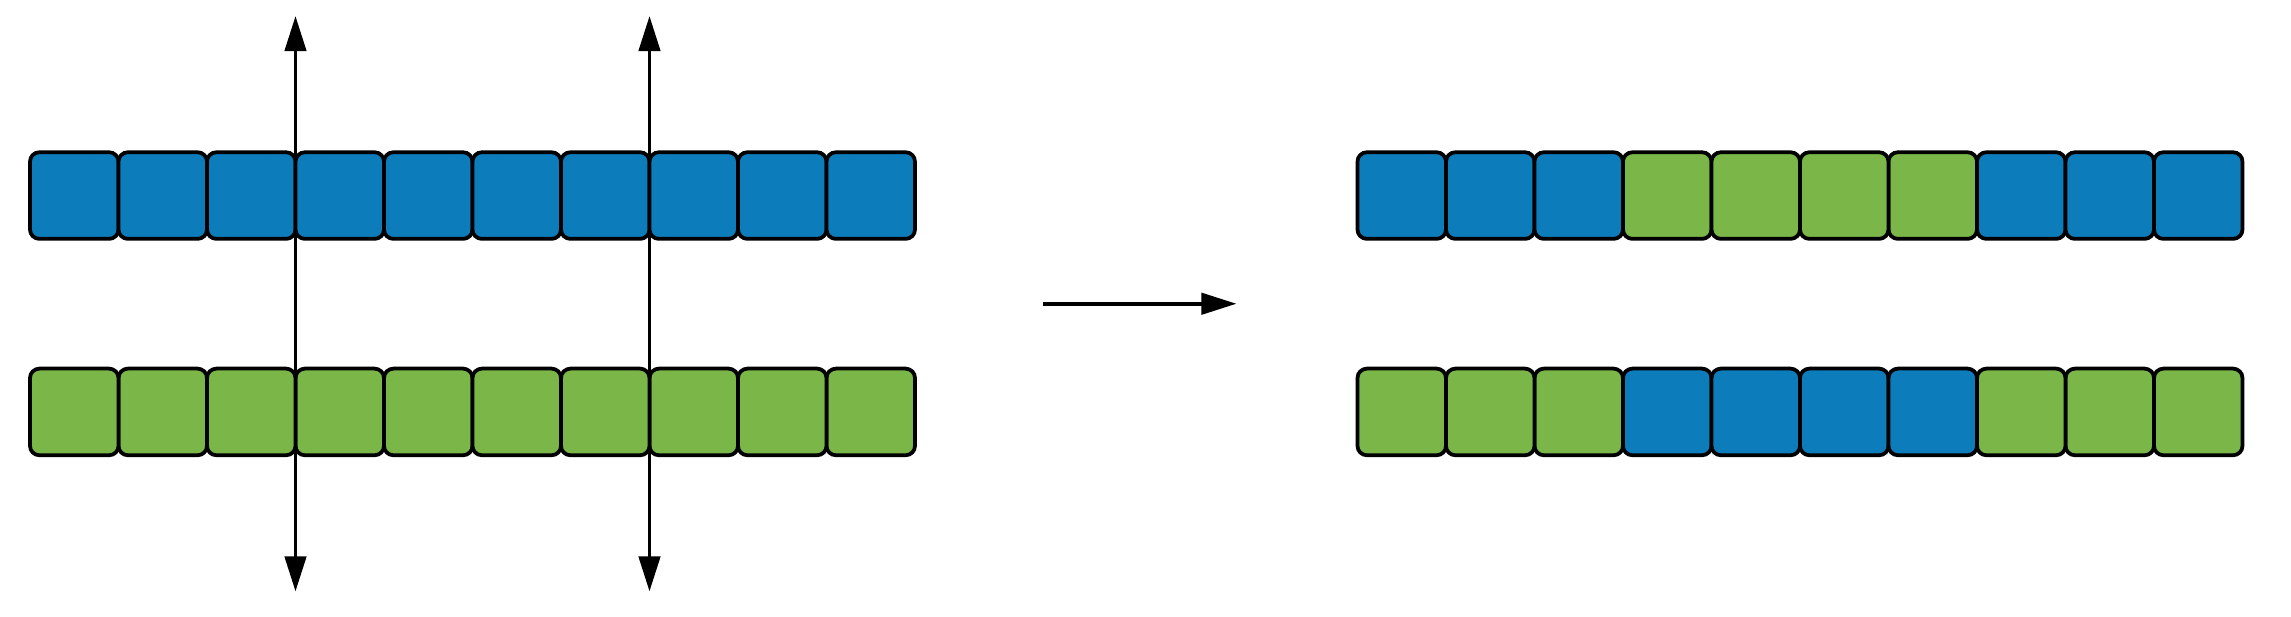
\includegraphics[width=1.0\textwidth]{crossover.png}
    \caption{Ação de crossover em dois pontos.}
    \label{fig:crossover}
\end{figure}

Toda ação bem sucedida de crossover gera duas sequências de genes (filhas) novas a partir das sequências originais (pais), as quais são transformadas em indivíduos e adicionadas à população.

O valor normalmente associado à variável $p_c$ na literatura costuma ficar sempre em torno de 0.9, valor padronizado neste trabalho. Tal valor precisa ser alto para que os filhos tenham maiores chances de variar seus genes ao longo das gerações.

\section{Mutação}

A ação de mutação atua sobre todos os genes da população (pais e filhos), a qual avalia, com probabilidade $p_m$, se a expressividade destes genes será alterada. Se sim, o valor deste gene é alterado de acordo com a assinatura de mutação do gene, tal como foi explicado no capítulo anterior. Normalmente, esta mudança de valor é aleatória.

O valor normalmente associado à variável $p_m$ na literatura costuma ser mais baixo, pois um valor muito alto não seria capaz de permitir a convergência das soluções. O valor padronizado neste trabalho foi de 0.01.

\section{Sobrevivência}

A ação de sobrevivência aqui também tentou ser relativamente simples. Os indivíduos (pais e filhos) após a mutação são ordenados de acordo com a função de fitness, e apenas os $\mu$ melhores indivíduos são mantidos. Ou seja, a população não aumenta de tamanho ao longo das gerações.

